\documentclass{article}
\usepackage[utf8]{inputenc}
\usepackage[margin=0.625in]{geometry}
\usepackage{parskip, setspace}
\setstretch{1.5}
\usepackage{amsmath, amsfonts}
%\numberwithin{equation}{subsection}
\usepackage{graphicx, caption, wrapfig}
\usepackage{hyperref}
\usepackage{multirow}

\usepackage{biblatex}
\addbibresource{bib.bib}

\renewcommand{\arraystretch}{1.5}

\title{\Large \vspace{-0.625in} Proposal for thesis titled \\ \emph{Production of massless spin-0 particles in analog (3+1)-dimensional de Sitter universes from a ground state BEC using high-performance computing} \vspace{-0.15in}}
\author{Nathaniel W. Chapman \\ {\normalsize Central Washington University}}
\date{\vspace{-0.1in}\today}

\begin{document}

    \maketitle
    
    \begin{center}
        Abstract \\
        During the moments just after the Big Bang, particles were produced due to the rapid expansion of the universe. Because direct observation of the universe at this time is impossible, a lab-based ultra-cold quantum gas can be used as an analog.  Previous research has been done to computationally model these gases while restricted to a quasi-two-dimensional geometry.  This restriction yields an analog universe with two only spatial dimensions and a description of a reduced momentum distribution of the created particles.  A computational model simulating an unrestricted gas and an analog universe with three spatial dimensions requires the use of high-performance computing.  I aim to use high-performance computing to simulate the full-dimensional system. This will allow me to measure the error associated with using a reduced-dimensional model, and determine the cost-benefit ratio to using a high-performance implementation.
        %\begin{itemize}
        %     \item Provide insight into the dynamics of particles created due to the expansion of the universe in the moments just after the Big Bang.
            
        %     \item Quantitatively describe the error in using a reduced-dimensional physical model as compared to a full-dimensional model.
            
        %     \item Quantitatively describe the balance between the costs and benefits of using a full-dimensional with high-performance computing.
            
        %     \item Provide an accessible, free, open-source, ``ready to use package'', high-performance computational model that can be used to investigate systems such as the one described here.
        % \end{itemize}
    \end{center}
    
    \section{Background}

        \subsection{Physical Background}

            Directly measuring the properties of the universe just after the Big Bang is impossible, as that was almost 14 billion years ago.  Even \emph{indirectly} measuring these properties is extremely difficult via traditional means.  During these brief moments just after the Big Bang, the universe expanded rapidly in a particular way.  During this expansion there were particles popping in and out of existence, each with its own dynamics (e.g. position and momentum).
    
            What is less difficult is cooling down gases to near absolute-zero (about a billion times colder than empty space).  Gases made of certain atoms or molecules have properties that can be changed to almost any value we want.  Because of this, we can turn our knobs in the lab to make the gas behave in a way that matches a certain mathematical model.
            
            For some types of gases, we can choose how strongly the particles in the gas interact with each other.  It turns out that we can choose a certain interaction strength so that the mathematical model that describes how the gas behaves \textbf{exactly} matches the mathematical model of how particles are produced in the universe in the moments just after the Big Bang!  When this happens, we can call this ultra-cold gas an ``analog universe''.

\pagebreak
    
            Because of this mathematical equality, we can effectively observe the particles in the moments just after the Big Bang, but in the lab. Moreover, these observations can be made using a tried-and-true system that has been developed and used over the past thirty years\cite{firstBEC}.
        
        %One of the aims of this thesis is to provide a high-performance computational model that allows researchers to reasonably investigate a full-dimensional system.  To maximize efficiency, this model will employ the use of high-performance techniques and hardware such as cluster and GPU computing using the CUDA massively parallel computing framework.  Purpose built scientific software libraries, such as the multi-GPU CUDA Fast Fourier Transform library, will be used.
        
    % b) Relationship to previous research/knowledge or creative activity in the field (literature review) including relationship to your previous work
    %\section{Context}
        % \begin{itemize}
        %     % \item Analogs aren't new
        %     % \item Acoustic analogs of bound quantum particles in infinite and Coulomb potential, me in Junior Lab
        %     % \item Acoustic black holes, proposed in '88 by Unruh, formalized in '98 by Visser
        %     % \item Thesis by Jain, 2017
        %     % \item Gravitational Analog Phenomenology, book
        %     % \item Cold Atom Laboratory on the ISS, by NASA
        %     %\item Nonlinear dispersion corresponds to breaking Lorentz invariance [Jain 23, 25, 26, 17]
        %     %\item Theoretical analogs for massive and spin-1 particles [26, 30-36]
        %     %\item Non-zero background velocity [3-7]
        %     %\item Particle production follows the standard methodology [1,2]
        %     %\item sudden transition for parametric oscillator [44]
        %     %\item sudden transition provides the maximal particle production [59]
        %     %\item Cyclic universe has also been studied [66]
        %     %\item Particle production for tanh expansion [8]
        %     %\item de Sitter expansion describes inhomogeneities observed in the universe [61]
        %     %\item Particle production in a de Sitter universe predicted by Hawking [62, 63]
        %     %\item Experimental control of interaction strength [8, 37, 38]
        %     %\item Experimental results from JILA showing Rubidium 85 as a promising candidate for experimental realization [79, 80]
        %     %\item Parameters, but with large $N_0$, from [76]
        % \end{itemize}

            Studies have investigated gases with
            
            \begin{itemize}
                \item phonons with a temporal frequency that is nonlinearly related to the spatial frequency (dispersion relation)\cite{Nonlinear_dispersion_Lorentz_breaking_1, Nonlinear_dispersion_Lorentz_breaking_2, Nonlinear_dispersion_Lorentz_breaking_3}
                
                \item analog massive particles\cite{massive_1, massive_2, massive_3}

                \item analog particles with non-zero spin\cite{massive_and_spin_4, massive_and_spin_5, massive_and_spin_6, massive_and_spin_7}

                \item analog universes with different expansion behavior\cite{sudden_transition_1, sudden_transition_2, cyclic_cosmology, Experimental_interaction_strength_1}

                \item analog universes with non-zero background velocity\cite{background_velocity_1, background_velocity_2, background_velocity_3, background_velocity_4, background_velocity_5}

                \item promising experimental realizations \cite{Experimental_candidate_1, Experimental_candidate_2, Experimental_interaction_strength_1, Experimental_interaction_strength_2}
            \end{itemize}

        \subsection{Computational Background}

            Computationally, simulations have had to investigate analog universes of reduced dimension due to the unreasonable time it takes to simulate full-dimensional systems without using high-performance computing.  These simulations have been deemed accurate enough as it is proposed that a full-dimensional simulation would yield qualitatively similar results.  In order to be confident in the level of accuracy of the reduced-dimensional simulations, those results need to be compared to those of a full-dimensional simulation.  This will not only allow a quantification of the error in the reduced-dimensional simulation, but also a measure of the error-to-resource efficiency of a full-dimensional simulation.
    
            Future insight into these analog systems and the fundamental properties of the early universe require computational support.  A readily-usable computational model will not only allow theoretical investigations to make predictions, but also allow experimental research to have a guide on where to go next and have something with which to compare.  The availability of this work is paramount to more efficient and more physically-accurate insight into our universe.

        \subsection{Foreground} \label{sec:Foreground}
            
            I choose a gas with linear dispersion, analog massless and spin-0 particles, an analog universe undergoing a de Sitter expansion with zero background velocity.  The de Sitter spacetime is chosen because of its significance to modern cosmology and previously predicted particle production (as done by Hawking)\cite{de_Sitter_inhomogeneities, de_Sitter_particle_production_1, de_Sitter_particle_production_2}. Particle production will be calculated with standard methods\cite{particle_production_1, particle_production_2}.  The numerical parameters chosen in this study also follow from previous studies\cite{parameters}.  Computational implementations will be done using high-performance methods.
\pagebreak
    \section{Goals} \label{sec:Goals}
        % \begin{itemize}
        %     \item Provide insight into how particle production fits into significant cosmological models
        %     \item Provide a computational model to support and guide theoretical and experimental investigations.
        %     \item Update previous with modernized code and computational methods.
        % \end{itemize}

        I aim to achieve several goals from studying this system: 
        
        \begin{enumerate}
            \item \textbf{Provide insight into the dynamics of particles created due to the expansion of the universe in the moments just after the Big Bang.}

                The behavior of particles created in the early universe are impossible to observe directly.  I aim to use the similarity between the physics of the early universe and the physics of ultra-cold condensed matter systems to describe the behavior of particles that existed 14 billion years ago.
            
            \item \textbf{Quantitatively describe the error in using a reduced-dimensional physical model as compared to a full-dimensional model.}  
            
                Previously developed models\cite{Jain} describe the spontaneous creation of particles in an expanding analog universe with two spatial dimensions that emerges from a quasi-two-dimensional ultra-cold gas.  I aim to determine the error in the previous model by comparing the results to those of a similar analog universe but with three spatial dimensions.
                
            \item \textbf{Quantitatively describe the efficiency of using a full-dimensional model with high-performance computing.}

                The developers of the previous model\cite{Jain} stated the results of a model considering three spatial dimensions would be qualitatively similar to those of the model with two spatial dimensions.  Combined with the error measured between the two models, I aim to describe if using high-performance methods is worth the extra effort, and by how much.
            
            \item \textbf{Provide an accessible, free, open-source, ``ready to use package'', high-performance computational model that can be used to investigate systems such as the one described here.}

                Upon completion, these new methods and implementation will be free and publicly available on the code-hosting website GitHub.  Such availability is an integral for open-access science and dissemination to future researchers needing support in their computer simulations.
                
        \end{enumerate}
        
    % d) Clear statement of methodology/research design or creative approach
    \section{Methods}
        % \begin{itemize}
        %     \item Computational implementation: numerical differential equation solver, FFT, numerical differentiation, and vectorized arithmetic
        %     \item high-performance computing platforms such as cluster, grid, or GPU computing.
        %     \iitem Use Mathematica or Julia or something faster if needed.
        % \end{itemize}

        \subsection{Physical Theory}

            The following physical model is for an analog universe with two spatial dimensions.

            \subsubsection{Setting up the Analog}

                The gas as is outlined in section \ref{sec:Foreground} is called a ground-state Bose-Einstein condensate (BEC) without thermal or quantum fluctuations.  \pagebreak The dynamics of this BEC are described by the Gross-Pitaevskii equation (GPE) under a Bogoliubov mean-field approximation (also known as the \textit{nonlinear Schr{\"o}dinger equation}),
                
                \begin{equation} \label{eq:GPE}
                    i \hbar \, \partial_t \psi(\mathbf{x}, t) = \left[ -\frac{\hbar^2}{2 m} \nabla^2 + V_\text{ext}(x) + U \left| \psi(\mathbf{x}, t) \right|^2 \right] \psi(\mathbf{x}, t).
                \end{equation}
                
                Using a linearized Madelung density-phase representation
    
                \begin{equation} \label{eq:Madelung}
                    \psi(\mathbf{x}, t) = \sqrt{n_0 + \hat{n}} e^{i \left( \theta_0 + \hat{\theta} \right)},
                \end{equation}
    
                where $n_0 + \hat{n}$ is the linearized form of the real density field $n(\mathbf{x}, t)$ and $\theta_0 + \hat{\theta}$ is the linearized form of the real phase field $n(\mathbf{x}, t)$, equation (\ref{eq:GPE}) becomes\cite{Jain} 
    
                \begin{equation} \label{eq:KG}
                    \frac{1}{\sqrt{-g}} \partial_\mu \left[ \sqrt{-g} g^{\mu \nu} \partial_\nu \hat{\theta} \right] = 0,
                \end{equation}
    
                where 
    
                \begin{equation} \label{eq:metric}
                    g_{\mu \nu} = \left( \frac{n_0}{c} \right)^{2 / (d - 1)} \begin{bmatrix}
                        -c^2 & \vdots & 0 \\
                        \cdots & & \cdots \\
                        0 & \vdots & \delta_{ij}
                    \end{bmatrix}
                \end{equation}
    
                can be interpreted as the covariant metric tensor (with determinant $g$) describing an analog, spatially flat, Friedmann–Lema{\^i}tre–Robertson–Walker universe, $c$ is the speed of sound in the condensate, and $d$ is the number of spatial dimensions.  \textbf{Equation (\ref{eq:KG}) describes both the phase-perturbations $\hat{\theta}$ of oscillations with low spatial frequency (i.e. low momentum phonons) in the BEC and also the dynamics of a quantum field that produces massless, spin-0 particles.}

            \subsubsection{Expanding Universes}

                The time dependence of the system is completely captured in the speed of sound by 
    
                \begin{equation} \label{eq:speed}
                    c(t)^2 = \frac{U(t) n_0}{m} = \frac{4 \pi \hbar^2}{m^2} n_0 a(t),
                \end{equation}
    
                with atoms of mass $m$, scattering length $a$, and number density $n_0$.  With the dimensionless scaling function $b(t)$, the interaction strength $U(t)$ (or equivalently the scattering length) has time dependence defined by 
    
                \begin{equation}
                    U(t) \equiv U_0 b(t),
                \end{equation}
\newpage
                where $U_0 = U(t_0)$ for an initial time $t_0$.  Then equation (\ref{eq:speed}) becomes 
    
                \begin{equation}
                    c(t) = c_0 \sqrt{b(t)}.
                \end{equation}
    
                This time dependence of the speed of sound and interaction strength allows us to draw another analogy.  If the speed of sound decreases with time, it would appear as if the space between the source and the observer were increasing.  Similarly, if the speed of sound increases with time, it would appear as if the space between the source and observer is decreasing. With this in mind, if the interaction strength between atoms $U(t)$ decreases with $t$, the analog universe is expanding, and if $U(t)$ increases, the analog universe is contracting.

            \subsubsection{The Field Equation}

                With the scaling function, equation (\ref{eq:KG}) becomes

                \begin{equation} \label{eq:fieldEquation}
                    \partial_\eta^2 \hat{\theta} - \frac{1}{2} \frac{\dot{b}(\eta)}{b(\eta)} \partial_\eta \hat{\theta} - c_0^2 \nabla^2 \hat{\theta} = 0,
                \end{equation}

                where $\eta$ is the conformal time defined by $d\eta = \sqrt{b(t)} dt$.  Equation (\ref{eq:fieldEquation}) governs the dynamics of oscillations in the BEC for a time-dependent speed of sound, and the behavior of the massless, spin-0 particles in an expanding universe.  Then we can expand the phase $\hat{\theta}(\mathbf{x}, t)$ and density $\hat{n}(\mathbf{x}, t)$ perturbation fields in a Fourier plane-wave amplitude representation as 

                \begin{subequations} \label{eq:FourierExpansion}
                \begin{equation}
                    \hat{\theta}(\mathbf{x}, t) = \frac{1}{\sqrt{V}} \sum_\mathbf{k} e^{i \mathbf{k} \cdot \mathbf{x}} \chi_\mathbf{k}(t) \hat{b}_\mathbf{k}(t) + e^{-i \mathbf{k} \cdot \mathbf{x}} \chi_\mathbf{k}^*(t) \hat{b}_\mathbf{k}^\dagger(t)
                \end{equation}
                \begin{equation}
                    \hat{n}(\mathbf{x}, t) = \frac{1}{\sqrt{V}} \sum_\mathbf{k} e^{i \mathbf{k} \cdot \mathbf{x}} n_\mathbf{k}(t) \hat{b}_\mathbf{k}(t) + e^{-i \mathbf{k} \cdot \mathbf{x}} n_\mathbf{k}^*(t) \hat{b}_\mathbf{k}^\dagger(t)
                \end{equation}
                \end{subequations}
                
                (Note: $\chi_\mathbf{k}(t)$ and $n_\mathbf{k}(t)$ are implicitly spatially dependent because they to the fields at a point in space) so that equation (\ref{eq:fieldEquation}) becomes

                \begin{equation} \label{eq:fieldEquationdeSitter}
                    \partial_\eta^2 \chi_\mathbf{k} - \frac{1}{\eta} \partial_\eta \chi_\mathbf{k} + c_0^2 k^2 \chi_\mathbf{k} = 0,
                \end{equation}

                where the scaling function $b$ has been defined such that $b(t) = e^{-t / t_s}$ so that the analog universe is undergoing a de Sitter type expansion on a time scale $t_s$.  The boundary conditions for equation (\ref{eq:fieldEquationdeSitter}) come from the fact that $\chi_\mathbf{k}$ needs to be continuous at the moment when expansion begins.

            \subsubsection{Particle Production} \label{sec:particleProduction}

                The number of particles $N_k(t)$ produced at time $t$ with wave vector $\mathbf{k}$ is described by the equation

                \begin{equation} \label{eq:particleProduction}
                    N_k(t) = \left| u_k^{\text{out} *}(t) v_k^{\text{exp} *}(t) - v_k^{\text{out} *} u_k^{\text{exp} *}(t) \right|^2
                \end{equation}

                where

                \begin{subequations} \label{eq:mixedFourierAmplitudes}
                \begin{equation}
                    u_k(t) = \frac{1}{2 \sqrt{n_0}} n_k(t) + i \sqrt{n_0} \chi_k(t)
                \end{equation}
                \begin{equation}
                    v_k(t) = \frac{1}{2 \sqrt{n_0}} n_k(t) - i \sqrt{n_0} \chi_k(t),
                \end{equation}
                \end{subequations}

                ``out'' and ``exp'' corresponding to regions of spacetime outside of and inside the expansion of the universe, and the density field Fourier plane wave amplitude is given by 

                \begin{equation} \label{eq:densityFromPhase}
                    n_\mathbf{k} = - \frac{\hbar}{U} \partial_t \chi_\mathbf{k}.
                \end{equation}

                It might help to summarize the entire process of calculating the particle production in steps. To calculate the number of particles produced at position $\mathbf{x}$ and time $t$ with wave vector $\mathbf{k}$ looks like the following:

                \begin{enumerate}
                    \item Solve the field equation (\ref{eq:fieldEquationdeSitter}) for $\chi_\mathbf{k}(t)$
                    \item Differentiate $\chi_\mathbf{k}(t)$ to get $n_\mathbf{k}(t)$ as in equation (\ref{eq:densityFromPhase})
                    \item Combine $\chi_\mathbf{k}(t)$ and $n_\mathbf{k}(t)$ as in equations (\ref{eq:mixedFourierAmplitudes})
                    \item Calculate the number of particles at time $t$ with wave vector $\mathbf{k}$ as in equation (\ref{eq:particleProduction})
                \end{enumerate}

            \subsubsection{Computational Parameters} \label{sec:parameters}

                The aforementioned previous model\cite{Jain} considered a system with several specified parameters.  The universe with had a size of 128 $\times$ 128 grid points. The length of time encompassed several different scales ranging from $10^{-5}$ to $10^{-3}$.  The domain of wave vectors whose norm is less than $32 \times 2 \pi$.  This domain of wave vectors resulted in 3209 values of $\mathbf{k}$, which corresponds to the number of terms in the Fourier expansions (eq. \ref{eq:FourierExpansion}) at each point in the field at each point in time.  Ultimately this leads to $3209 \times 128 \times 128 \approx 5 \times 10^7$ values of $\chi_\mathbf{k}$ for a single moment in time.  The time step was chosen such that the total particle number for the entire field changed by much less than one.

                \begin{table}[h]
                    \centering
                    \begin{tabular}{c|c}
                        \multicolumn{2}{c}{Previous domains}  \\
                         Universe Size $\mathbf{x}$      & 128 $\times$ 128 \\
                         \hline
                         Time Scale $t_s$                & $10^{-5}$ to $10^{-3}$ \\
                         \hline
                         Wave Vector Domain $\mathbf{k}$ & $||\mathbf{k}|| \leq 32 \times 2 \pi$ \\
                    \end{tabular}
                    \quad
                    \begin{tabular}{c|c}
                        \multicolumn{2}{c}{New domains}  \\
                         Universe Size $\mathbf{x}$      & $128 \times 128 \times 128$ \\
                         \hline
                         Time Scale $t_s$                & $10^{-5}$ to $10^{-3}$ \\
                         \hline
                         Wave Vector Domain $\mathbf{k}$ & $||\mathbf{k}|| < k_c$ \\
                    \end{tabular}
                    \caption{Previous and new computational domains}
                    \label{tab:Domains}
                \end{table}

                I will extend these domains to include a universe with three spatial dimensions, starting with a cubic grid of $128 \times 128 \times 128$, and all wave vectors that are valid in the system I have described i.e. all wave vectors with $||\mathbf{k}|| \leq k_c$ where $k_c$ is defined such that $\hbar^2 k_c^2 / 2 m = U n_0$.

        \subsection{Computational Methods}

            The computational choices that need to be made are: the numerical algorithms, the high-performance hardware, and the programming language.  The biggest influence on these choices is the level of desired performance.  All the relevant numerical algorithms have different forms that balance speed and accuracy, such as the order of a Runga-Kutta derivative.  The high-performance hardware could range in performance from a loosely cluster of CPUs to a ``tight'' cluster of high-performance GPUs, but the implementation on the GPU cluster would require a dedicated implementation possibly using the CUDA parallel computing framework.  Different programming languages offer different amounts of performance, balanced by the amount of effort it takes to implement the algorithms.

            \subsubsection{Algorithms \& Hardware}

                I will use conventional methods to perform the actions outlined at the end of section \ref{sec:particleProduction}.  I plan to solve the field equation (eq. \ref{eq:fieldEquationdeSitter}) using a fourth-order Runga-Kutta method, mirroring previous implementations\cite{Jain}.  Transforming the phase field Fourier amplitudes to those of the density field (eq. \ref{eq:densityFromPhase}) will be done with a fourth-order accurate central finite difference.  Finally the particle production for all $k$ at a certain time (eqs. \ref{eq:particleProduction}, \ref{eq:mixedFourierAmplitudes}) will be calculated in using vectorized and/or parallel methods.
    
                \begin{table}[h]
                    \centering
                    \begin{tabular}{c|c}
                        Physics & Method \\
                        \hline
                        Fourier Field Equation & 4-th order Runga-Kutta \\
                        \hline
                        Density-Phase Transformation & 4-th order Central FD \\
                        \hline
                        Particle Production & Vectorized Arithmetic
                    \end{tabular}
                    \caption{Computational methods that will be used for each step in the calculation of particle production}
                    \label{tab:methods}
                \end{table}
    
                On the choice of high-performance hardware, I plan to use the IBM high performance computing cluster (a.k.a ``Turing'') owned by the CWU College of the Sciences.  As this platform is running the Ubuntu Linux operating system and consists of a cluster head-node, a cluster storage node and 4 cluster compute nodes which contain NVIDIA GPU hardware, it fits my considerations on compute capability and hardware needs for cluster GPU computing using CUDA.  Other platforms that could be utilized are the ``loose cluster'', owned by CWU Information Services, or a custom configuration.

            \subsubsection{Programming Language}

                I expect to build this model using the Wolfram Language (also known as Mathematica) due to my knowledge and experience with it.  Though, since I am striving for wide distribution and open-access science, the free, open-source, modern, scientific programming language Julia is another quality candidate.  Both languages natively support high-performance implementations, with Julia having parallel computing as one of its fundamental considerations, as well as the ability to interface with cluster implementations and the CUDA GPU parallel computing platform.  If even more performance is needed, then other high-performance languages such as C++ or Java could be used.
    
                Then there is the point of reproducibility.  The Wolfram Language and the kernel in which runs is closed-source, and many of the native commands automatically choose the underlying method to use (e.g. the user does not know exactly how the Wolfram Language numerically solves a differential equation when using NDSolve.).  This prevents confident reproduction by other parties in future investigations or verifications.  Julia and other open-access languages do not have this restriction and thus would be more in-line what is generally considered ``good science''.
    
    % e) Timeline of research/creative activity for successful completion of the project
    \section{Timeline}
        % \begin{itemize}
        %     \item Extend the theoretical model from two dimensions to three dimensions over the summer of 2023
        %     \item Implement high-performance methods during fall 2024
        %     \item Write thesis and prepare journal ready publication during winter and spring quarters 2024.
        % \end{itemize}

        The expected timeline of this project will cover several phases over the next year.

        \subsection{Performance Scaling Phase - Summer '23}
        
            \begin{enumerate}
                \item Convert hybrid analytic-numerical algorithms to fully numeric low-performance algorithms (LPNA) in final language of choice
                \item Test the LPNAs in the 2D model and compare against previous results\cite{Jain}
                \item Translating the LPNAs to high-performance fully-numerical algorithms (HPNA) that make use of high-performance hardware
                \item Test the HPNAs in the 2D model and compare against previous results, measuring the efficiency when compared to the LPNA
            \end{enumerate}

        \subsection{Domain Scaling Phase - Fall '23}

            \begin{enumerate}
                \item Convert 2D theory to 3D
                \item If not generalized, convert the 2D HPNAs to 3D
                \item Test the 3D HPNAs on a small spatial domain and small momentum domain
                \item Test the 3D HPNAs on a small spatial domain and large momentum domain
                \item Do the ``real'' run of the 3D HPNAs on a large spatial domain and large momentum domain
                \item Revise and repeat runs until satisfactory results are achieved.
            \end{enumerate}

        \subsection{Writing Phase - Winter '24}

            \begin{enumerate}
                \item Write report
                \item Prepare for conferences
            \end{enumerate}

        \subsection{Dissemination Phase - Spring '24}

            \begin{enumerate}
                \item Defend thesis
                \item Present at conferences
                \item Submit final document to be considered for journal publication and graduation
            \end{enumerate}

        The adherence to this schedule is contingent upon sufficient funding and time during Summer '23.  If there are inadequate resources during this time, the performance scaling phase will need to be delayed.
        
    \section{Anticipated Results}

        The results I anticipate follow most of the goals outlined in section \ref{sec:Goals}.

        \begin{enumerate}
            \item \textbf{Goal: Provide insight into the dynamics of particles created due to the expansion of the universe in the moments just after the Big Bang.}

            \underline{\textbf{Expected Result}}

                As mentioned, the developers of the previous model upon which this research is based\cite{Jain} have stated that the results from a simulation considering a universe with three spatial dimensions should yield qualitatively similar results.  I have derived the field equations with respect to the lab time (not the conformal time) for two and three spatial dimensions to be 

                \begin{subequations}
                \begin{equation}
                    \text{2D: } \partial_t^2\theta - \frac{3}{2} \frac{b^\prime(t)}{b(t)} \partial_t \theta - c_0^2 b(t) \nabla^2\theta = 0
                \end{equation}
                \begin{equation}
                    \text{3D: } \partial_t^2\theta - \phantom{\frac{3}{2}} \frac{b^\prime(t)}{b(t)} \partial_t \theta - c_0^2 b(t) \nabla^2\theta = 0
                \end{equation}
                \end{subequations}

                These equations only differ in the constant coefficient to the first derivative i.e. the dissipative term.  Specifically, the two-dimensional field equation has a dissipative constant coefficient of 3/2 while the three dimensional field equation has a dissipative constant coefficient of 1.  Because of this small dissimilarity, I agree with the previous statement that a three-dimensional simulation should lead to qualitatively similar results.
            
            \item \textbf{Quantitatively describe the error in using a reduced-dimensional physical model as compared to a full-dimensional model.}
            
                \underline{\textbf{Expected Result}}

                Because the results of the new simulations should be qualitatively similar to those of the previous, I expect the error of the previous results to be small.  Though, this magnitude could range from negligibly small to ``small but significant''.  The conclusion from the former would be that the model using a universe with two-spatial dimensions is a good approximation to a full dimensional model, much like how a truncated Taylor series is a good approximation while the argument is small enough.  The conclusion from the latter would be that the low-dimensional model is ``unstably accurate'' in the sense that any \emph{further} approximations would yield a significantly poor approximation to the full dimensional model.
                
            \item \textbf{Quantitatively describe the efficiency of using a full-dimensional model with high-performance computing.}

                \underline{\textbf{Expected Result}}

                To show the computational efficiency of the analytic two-dimensional model via a ``naive'' implementation, I have recreated some of the results and figures from the previous model\cite{Jain} as shown in figures \ref{fig:finalTime} and \ref{fig:allTime}.  These calculations were done in the Wolfram Language on ``low-performance'' hardware.  Because these calculations were extremely fast on modern equipment, I believe that the worth of simulating a three-dimensional system on high-performance hardware will depend on the size of the domains as in section \ref{sec:parameters}.

                \begin{figure}[h]
                    \centering
                    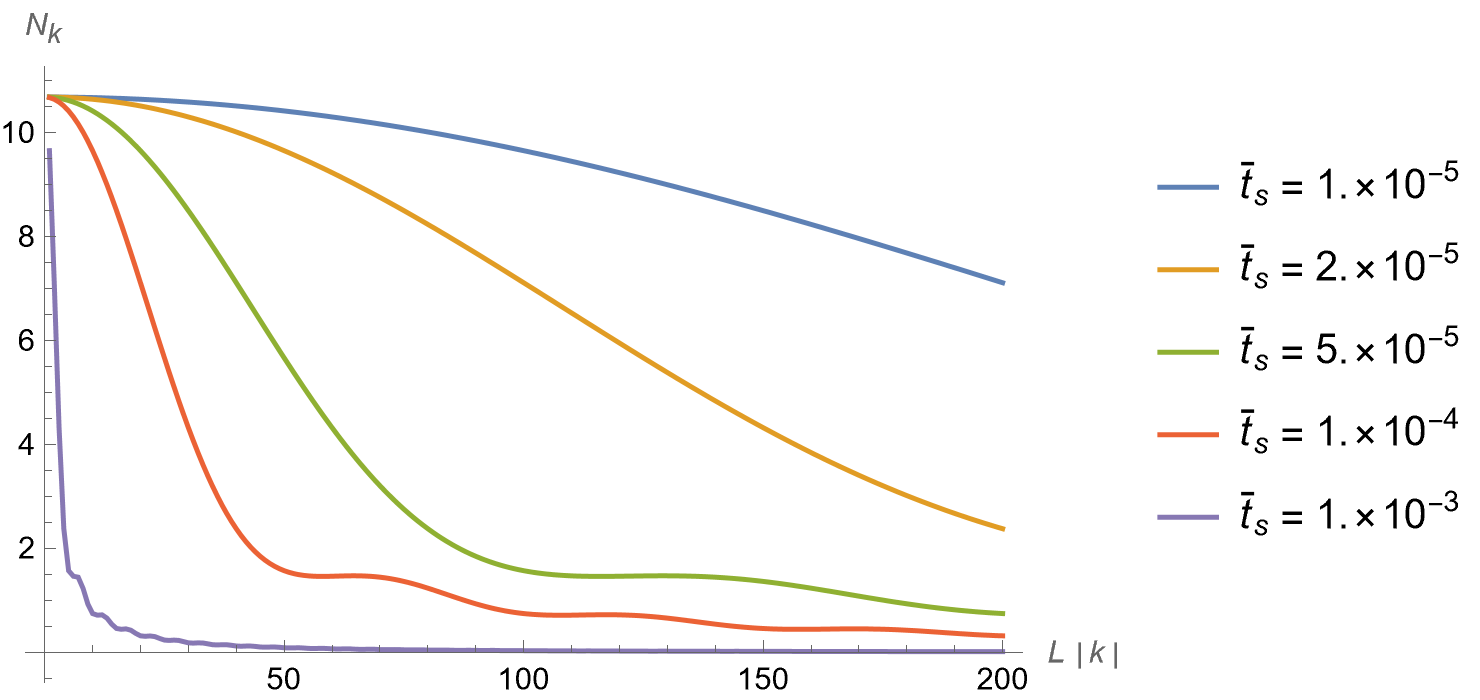
\includegraphics[width = 0.7\textwidth]{fig2.png}
                    \caption{The momentum distribution when the universe stops expanding for multiple effective rates of expansion}
                    \label{fig:finalTime}
                \end{figure}

                \begin{figure}[h!]
                    \centering
                    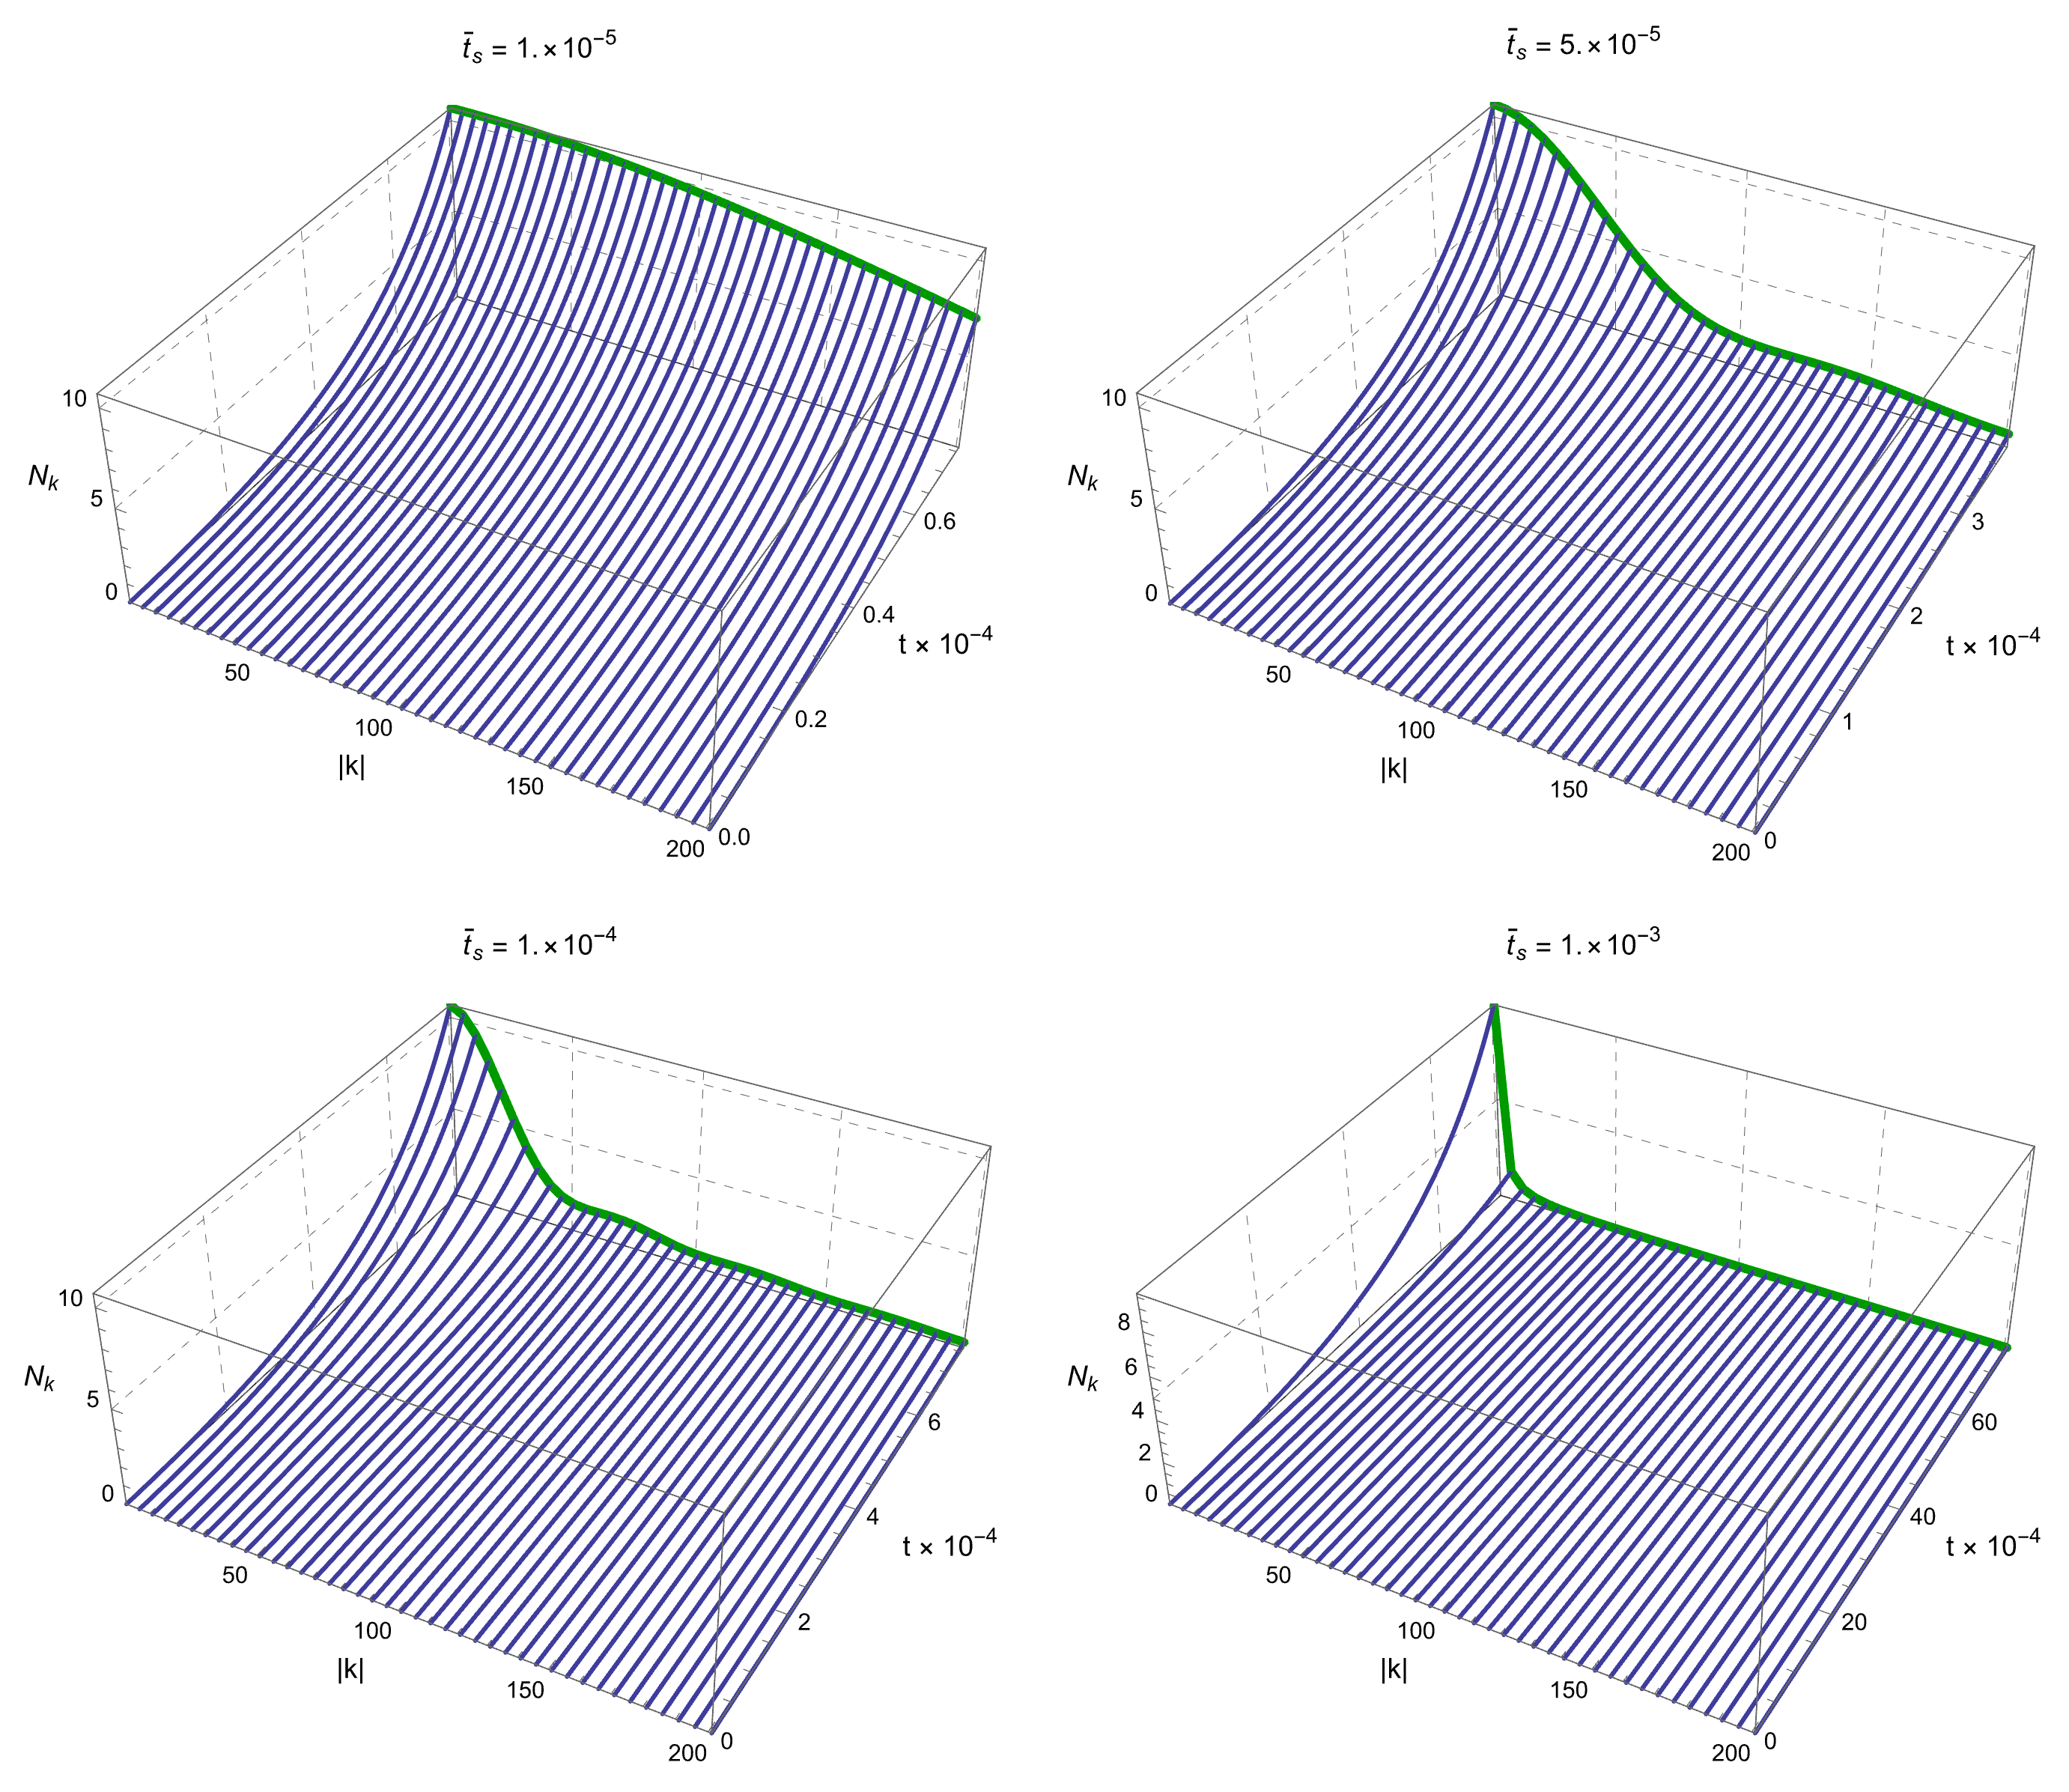
\includegraphics[width=\textwidth]{Analytic_Fig_4.png}
                    \caption{Momentum distribution throughout the expansion}
                    \label{fig:allTime}
                \end{figure}
                
        \end{enumerate}

        % This work aims to produce several results in different facets.  From a physical perspective, we will produce the data to describe particle production in a universe undergoing a de Sitter expansion.  From an efficiency approach, we will quantitatively describe the ratio of accuracy to ``effort'' in order for future investigations to determine if using the lower-dimensional model is sufficient for their needs.  From an accessibility viewpoint, we will produce a modern, open-source, and ready-to-use computational model that is available to future investigations.

        % The particle production data will be used to show how many particles have a specific momentum at a certain time during the expansion.  Additionally, the data will be used to show how that momentum distribution changes throughout the time in which the expansion is happening.  These figures will be intended to closely follow those found in previous investigations\cite{Jain}.

        % Because previous investigations were less accurate but needed fewer computational resources and time, these results will be used to assess the efficiency of the two-dimensional model.  In other words, we aim to provide a quantitative description of whether or not the increased accuracy of the three-dimensional model warrants the extra theoretical and computational effort as compared to the two-dimensional model\cite{Jain}.

        % The final result of this work will be a packaged software that can be downloaded and used ``out of the box'', for free, by anyone that can run the program.  This level of accessibility is meant to disseminate this work to everybody that wants it.
        
    % g) Plans for dissemination - this should also include an assessment of the potential for the project to lead to external funding.
    \section{Dissemination}

        After completion of the computational model, dissemination of the results will follow several paths.  This work is going to be presented as a ``journal ready thesis'' to be submitted to the American Physical Society's journal \textit{Physical Review D} covering particles, fields, gravitation, and cosmology.  I aim for further dissemination to come in the form of presenting at several conferences such as CWU's \textit{SOURCE}, the annual meeting of the American Physical Society's \textit{Northwest Section}, and, if resources permit, the American Physical Society's \textit{April Meeting} covering astrophysics, particle physics, nuclear physics, and gravitation.
    
    % h) CitedliteratureorReferences(notincludedin 8-pagelimitation)
    \pagebreak
    \nocite{*}
    \printbibliography

\end{document}
